\documentclass[12pt]{article}

\usepackage{amsfonts,amssymb}
\usepackage[utf8]{inputenc}
\usepackage[russian]{babel}
\usepackage{graphicx}
\usepackage{amsmath}
\usepackage{amsfonts}
\usepackage[ruled, lined]{algorithm2e}

\textheight=220mm
\textwidth=160mm

\newcommand{\sgn}{\operatorname{sgn}}
\newcommand{\argmax}{\operatorname{argmax}}
\newcommand{\NA}{\operatorname{NA}}
\newcommand{\OR}{\operatorname{ or }}
\newcommand{\LCS}{\operatorname{LCS}}
%\DeclareMathOperator{\sgn}{sgn}

\title{\bf Домашнее задание по курсу \\ <<Методы
и структуры данных поиска.>>}
\author{А.Е. Оразаев}
\date{}
\begin{document}

\voffset=-20mm
\hoffset=-12mm
\font\Got=eufm10 scaled\magstep2 \font\Got=eufm10

\maketitle

\section{Задача 3-4.}
\paragraph{Описание алгоритма.}
Для решения задачи несколько модифицируем алгорит Укконена для построения
суффиксных деревьев.

В каждой вершине $ v $ суффиксного дерева будем хранить также $ L_{v} $
длину префикса определяемого текущей вершиной для своего суффикса. Простыми
словами: глубину графа выраженную в символах, а не в вершинах.

Введем следующую модификацию в алгоритм: каждый раз, добавляя новую вершину
в дерево будем заполнять соответствующее поле массива $ l $, с результатами
работы алгоритма. Делать это будем вот так.

Перед началом алгоритма построения суффиксного дерева заполним весь массив
$ l $ нулями.

Пусть на шаге $ i + 1 $ нам встретился символ $ T[i + 1] = x $ и на
этом шаге нам стоит добавить вершину $ v $ в дерево. Заметим,
что у нас уже есть построенное суффиксное дерево $ ST_i $, которое выглядит
следующим образом.
\begin{center}
    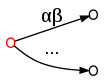
\includegraphics[width=60bp]{before_addition.png}
\end{center}

После добавления вершины дерево изменится следующим образом:
\begin{center}
    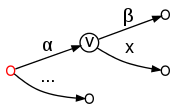
\includegraphics[width=100bp]{after_addition.png}
\end{center}

Здесь $ \alpha $ может быть не просто дугой, а путем из нескольких дуг до
вершины $ v $, при этом также $ \alpha $ может оказаться пустым путем, если
мы добавляем вершну $ v $ к корню, впрочем как и $\betta$ в этом случае.

Далее мы пологаем $ l_{i - |\alpha| + 1} = |\alpha| $, где $ |\alpha| = L_v $.
То есть отмечаем, что в позиции $ j = i - |\alpha| + 1 $,  $ \alpha $ --
наибольшая по длинне подстрока входного текста $ T $, начинающаяся в
позиции $ j $, которая также ранее встречается в $ T $.

Утверждается, что алгоритм Укконена с введенной модификацией вычисляет
искомый массив $ l $, для текста $ T $. С поправкой на то, что в конец
текста надо добавить сэнтинел $\$$. Но это уже деталь реализации.


\paragraph{Доказательство.}
Доказательство приведено во 2-ой лекции.






\paragraph{Сложность}
% FIXME: write complexity
Сложность по времений $ O(N) $.
Сложность по памяти $ O(N) $.

\end{document}
